\subsection{Exact Threshold Sensitivity and Available Headroom}
\label{app:threshold_headroom}

This post-hoc analysis reuses the original 110 units for each of the seven portfolios in Table~\ref{tab:equal_budget}. For a fixed portfolio $P$, define its available headroom as $H_P=R_P(\mathrm{always\mbox{-}graph})$, where $R_P$ is mean full-set regret against that portfolio's own graph/MLP oracle. Because regret is nonnegative, $H_P$ is an upper bound on any policy's absolute regret reduction relative to always-graph on these fixed outcomes. For $H_P>0$, the fraction closed by a policy $\pi$ is $(H_P-R_P(\pi))/H_P$; a negative fraction means the policy is worse than the reference. A small headroom limits the size of a possible improvement, not its existence or practical relevance.

We evaluate the family $\pi_t(h_1)=\mathrm{graph}$ if $h_1\geq t$ and MLP otherwise, with $t\in[0,1]$. Enumerating every interval between distinct observed homophily values, including the endpoints, covers every attainable decision pattern in this family. For sorted distinct values $v_1<\cdots<v_m$, these intervals are $[0,v_1]$, $(v_j,v_{j+1}]$, and $(v_m,1]$ when nonempty. The minimum uses all test outcomes to select $t$: it is an empirical lower bound on regret within this cutoff family, or equivalently an optimistic upper bound on its improvement. It is not an estimate of deployment performance, and does not replace the held-out calibration in Section~\ref{sec:calibrated_threshold}.

\begin{table}[ht]
\centering
\caption{Post-hoc headroom and exact test-selected cutoff minimum. Regrets are percentage points, averaged equally over the 11 datasets. All six single architectures are reported; each row has its own oracle. The final column is the fraction of headroom closed by the best cutoff, not a held-out improvement estimate.}
\label{tab:threshold_headroom}
\small
\begin{tabular}{@{}lrrr@{}}
\toprule
Graph action & Headroom & Minimum cutoff regret & Headroom closed (\%) \\
\midrule
Six architectures & 0.256 & 0.256 & 0.00 \\
GAT & 6.346 & 0.678 & 89.32 \\
GCN & 5.292 & 0.812 & 84.67 \\
GPR-GNN & 0.889 & 0.452 & 49.18 \\
GraphSAGE & 0.376 & 0.376 & 0.00 \\
H2GCN & 0.134 & 0.134 & 0.00 \\
LINKX & 2.133 & 2.133 & 0.00 \\
\bottomrule
\end{tabular}
\end{table}

Table~\ref{tab:threshold_headroom} and Figure~\ref{fig:threshold_headroom} separate threshold sensitivity from available improvement. For the full portfolio, the minimum is attained for $0\leq t\leq0.0446496653$ (upper endpoint rounded), yielding the always-graph actions. Thresholds 0.4, 0.5, 0.6, and 0.7 all yield 7.457 points because they fall in the same observed homophily gap, whose endpoints are approximately 0.3847711 and 0.7124682; $t=0.3$ yields 5.962. For GCN and GAT, the exact optimal interval is approximately $(0.2215615020,0.2219691047]$, giving lower minima than a 0.01-spaced grid. The supplement preserves full-precision intervals, all curve values, and the original-policy headroom fractions. This descriptive envelope changes neither the frozen cutoff nor the primary comparison family, and does not generalize to other diagnostics, richer policies, or unseen datasets.

\begin{figure}[p]
\centering
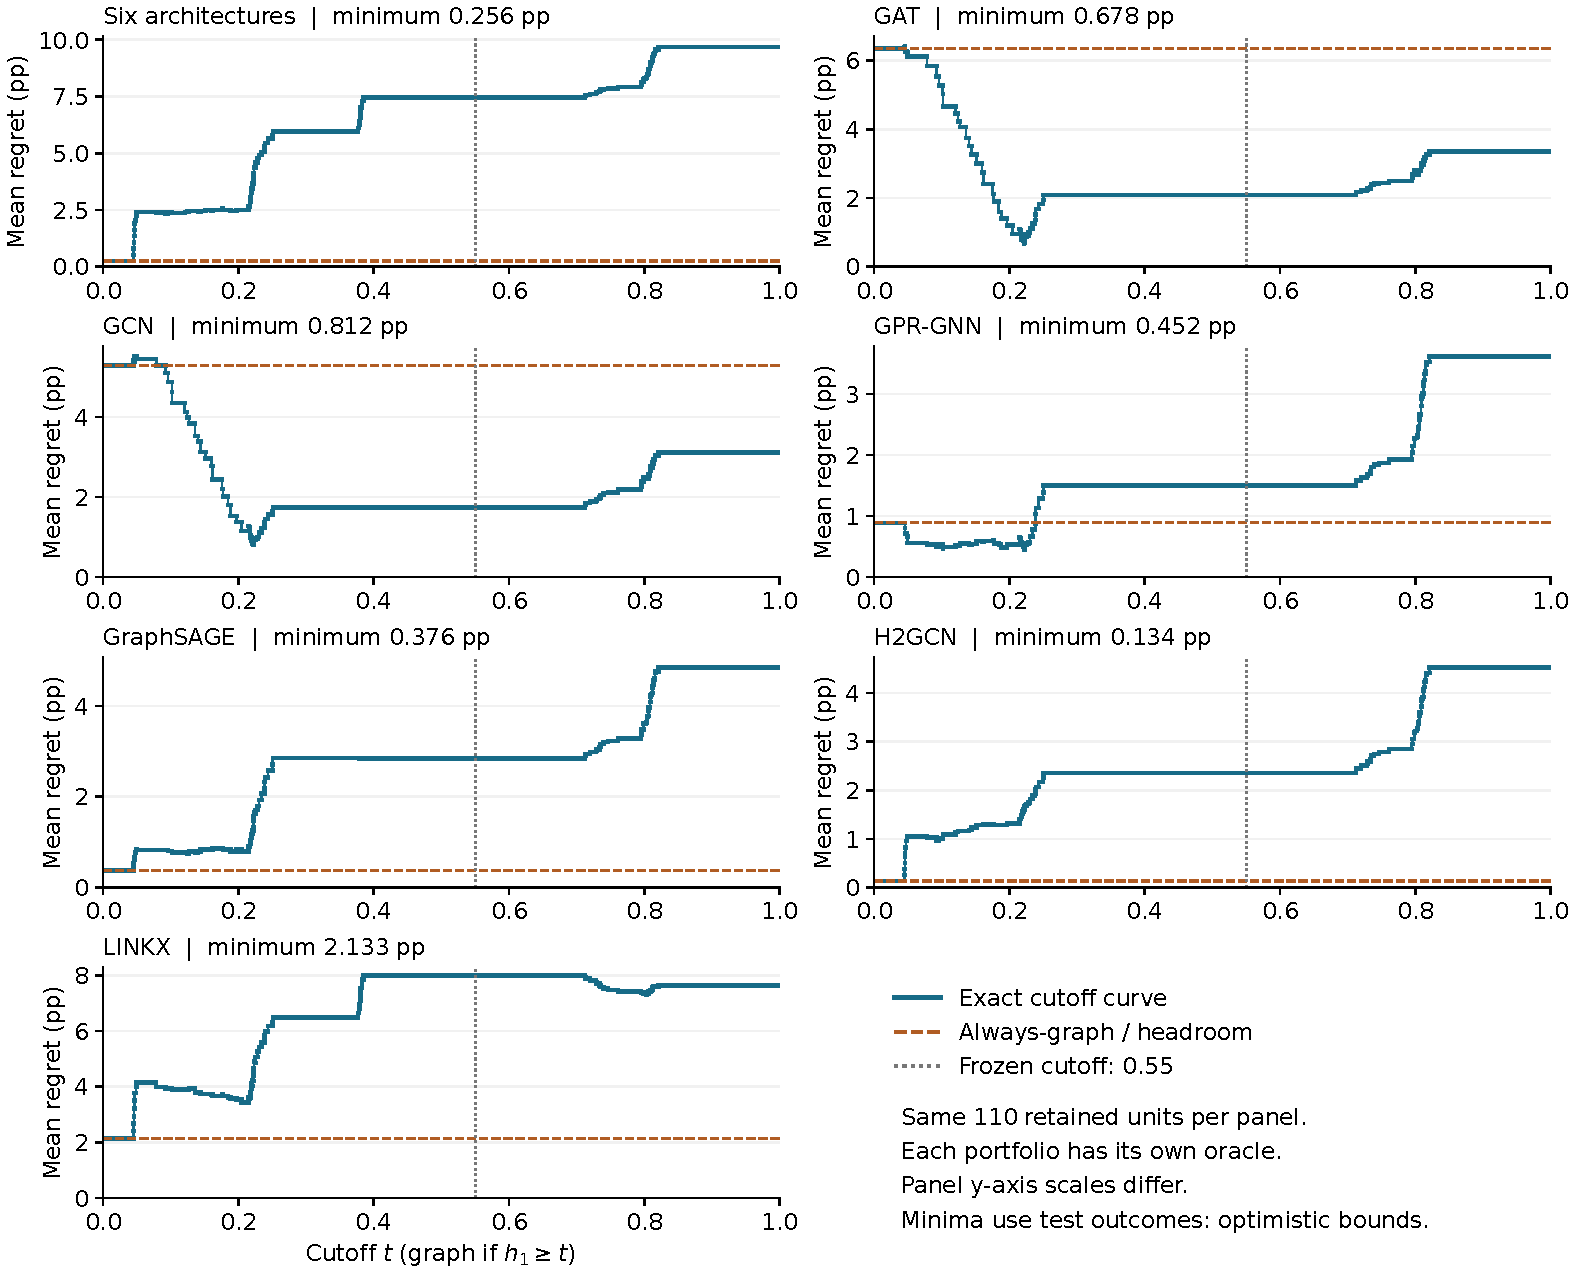
\includegraphics[width=\linewidth]{results/diagnostic/route_a_prospective_v2/analysis/threshold_headroom.pdf}
\caption{Exact one-sided homophily-cutoff curves from retained outcomes. The curves are constant on intervals ending at observed homophily values: equality selects graph. Vertical connectors guide the eye; full-precision endpoint inclusion is recorded in the supplement. Dashed horizontal lines show always-graph regret and dotted vertical lines show the frozen cutoff. Minima are selected using test outcomes, not held-out calibration. Panel vertical scales differ.}
\label{fig:threshold_headroom}
\end{figure}

\subsection{Action Counts and Raw Regret}
\label{app:action_confusion}

Table~\ref{tab:action_confusion} separates the practical-margin target from raw regret for the original full portfolio. The target is graph only when its test advantage exceeds one percentage point; raw regret instead measures any accuracy loss relative to the better recorded action. Thus a target-consistent MLP decision can still incur positive regret for a sub-margin graph advantage. The 19 and 30 graph-target counts are not the counts of positive-regret units, which are 23 and 32. All 40 explicit graph actions have zero regret in these records. This locates the observed policy losses without asserting that the rule cannot err when choosing graph in another setting.

\begin{table}[ht]
\centering
\caption{Full-portfolio action decomposition before the declared MLP fallback. Targets use the one-point margin; positive-regret counts use the raw accuracy difference. The contribution column divides each group's regret sum by all 110 units, so the entries add to the 7.457-point full-set regret.}
\label{tab:action_confusion}
\small
\begin{tabular}{@{}lrrrrr@{}}
\toprule
Action & Units & Graph target & MLP target & Positive regret & Contribution (pp) \\
\midrule
Graph & 40 & 40 & 0 & 0 & 0.000 \\
MLP & 35 & 19 & 16 & 23 & 1.799 \\
Abstain $\to$ MLP & 35 & 30 & 5 & 32 & 5.658 \\
\midrule
Total & 110 & 89 & 21 & 55 & 7.457 \\
\bottomrule
\end{tabular}
\end{table}
